\graphicspath{{./Imagenes/03/}}

\chapter{Marco Teórico}

Las ecuaciones resueltas en los experimentos numéricos trabajados en la Sección \ref{chap:06_resultados} provienen de la solución de sistemas mecánicos elastolineales, por ello conviene introducir la nomenclatura que se utilizará en el presenta trabajo

\section{Ecuaciones de elasticidad lineal}

\begin{figure}[h]
    \centering
    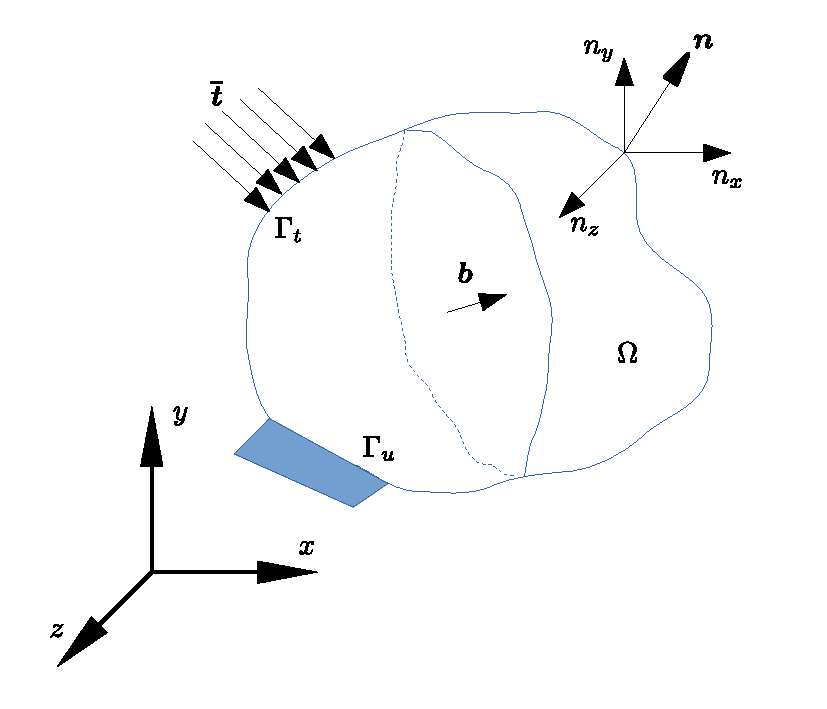
\includegraphics[width=0.8\textwidth]{sistema.pdf}
    \caption{Sistema mecánico general} \label{fig:sistema_general}
\end{figure}

Se tiene un sistema sólido continuo con dominio interior $\Omega$ y contorno $\Gamma = \Gamma_u \cup \Gamma_t$ donde $\Gamma_u$ y $\Gamma_t$ corresponde a los contornos donde preescriben condiciones de Dirichlet y Neumann respectivamente como se muestra en la Figura \ref{fig:sistema_general}, utilizando la notación de Voigt, el estado de esfuerzos $\bm{\sigma}$ sobre un sistema mecánico puede expresarse como 
\begin{equation}
    \bm{\sigma}^T = \left\{ \sigma_{xx} \; \sigma_{yy} \; \sigma_{yz} \; \sigma_{xz} \; \sigma_{xy} \right\}
\end{equation}
de igual manera, la deformación $\bm{\epsilon}$ se denota como
\begin{equation}
    \bm{\epsilon}^T = \left\{ \epsilon_{xx} \; \epsilon_{yy} \; \epsilon_{zz} \; \epsilon_{yz} \; \epsilon_{xz} \; \epsilon_{xy} \right\}
\end{equation}
La relación deformación-desplazamiento que permite describir $\epsilon$ en función del desplazamiento $\bm{u}$ viene dado por
\begin{equation} \label{eq:strain-displacement}
    \bm{\epsilon} = \bm{L} \: \bm{u}
\end{equation}
donde el vector desplazamiento está dado por el vector
\begin{equation}
    \bm{u}^T = \left\{ u \; v \; w \right\} 
\end{equation}
y el operador diferencial de la ecuación corresponde a
\begin{equation}
    \bm{L} = \begin{bmatrix} 
                       \partial/\partial x & 0 & 0 \\
                       0 & \partial/\partial y & 0 \\
                       0 & 0 & \partial/\partial z \\
                       0 & \partial/\partial z & \partial/\partial y \\
                       \partial/\partial z & 0 & \partial/\partial x \\
                       \partial/\partial y & \partial/\partial x & 0 
             \end{bmatrix}
\end{equation}
La ecuación constitutiva para fenómenos de deformación elasticolineal permite relacionar el estado de esfuerzos $\sigma$ con la deformación $\epsilon$ mediante la Ley Generalizada de Hooke, la que establece que:
\begin{equation} \label{eq:ley_de_hooke}
    \bm{\sigma} = \bm{D} \bm{\epsilon}
\end{equation}
En particular, para materiales isotrópicos la maatrix $\bm{D}$ resulta
\begin{equation}
    \bm{D} = \begin{bmatrix}
        D_{11} & D_{12} & D_{12} & 0 & 0 & 0 \\
               & D_{11} & D_{12} & 0 & 0 & 0 \\
               &        & D_{11} & 0 & 0 & 0 \\
               &        &        & G & 0 & 0 \\
               &  sim.  &        & & G & 0 \\
               &        &        & & & G
             \end{bmatrix}
\end{equation}
donde
\begin{equation}
    D_{11} = \frac{E(1-v)}{(1-2v)(1+v)} \; ; \; D_{12} = \frac{Ev}{(1-2v)(1+v)} \; ; \; G = \frac{D_{11}-D_{12}}{2} = \frac{E}{2(1+v)}
\end{equation}
En el cual $E$ es el módulo de Young, $v$ es el coeficiente de Poisson y $G$ es el módulo de corte.

La ecuación de equilibrio mecánico está dado por la siguiente expresión
\begin{equation} \label{eq:equilibrio_mecanico}
    \bm{L}^T \bm{\sigma} + \bm{b} = \rho \ddot{\bm{u}} + c \dot{\bm{u}}
\end{equation}
Donde $\rho$ es la densidad de masa, $c$ es el coeficiente de amortiguamiento, $dot{\bm{u}} = \partial u/\partial t$ es el vector velocidad, $\ddot{\bm{u}} = \partial^2 u/\partial t^2$ es el vector aceleración y $\bm{b}^T = \left\{ b_1 \; b_2 \; b_3 \right\}$ es la fuerza de cuerpo ejercida sobre el sistema. Reemplazando las ecuaciones \ref{eq:strain-displacement} y \ref{eq:ley_de_hooke} en \ref{eq:equilibrio_mecanico} y suponiendo un sistema estacionario $(\dot{\bm{u}} = \ddot{\bm{u}} = \bm{0})$  se obtiene:
\begin{equation}
    \bm{L}^T \bm{D} \bm{L} \bm{u} + \bm{b} = \bm{0}
\end{equation}
La cual está sujeta a las canciones de borde las que se pueden clasificar de la siguiente manera:
\begin{align}
    \mbox{Tracción preescrita (Neumann): } & \bm{\sigma} \cdot \bm{n} = \overline{\bm{t}} & \bm{x} \in \Gamma_t &  \\
    \mbox{Desplazamiento preescrito (Dirichlet): } & \bm{u} = \overline{\bm{u}} & \bm{x} \in \Gamma_u &  \\
    \mbox{Desplazamiento inicial: } & \bm{u}(\bm{x},t_0) = \bm{u}_0 (\bm{x}) & \bm{x} \in \Omega &  \\
    \mbox{Velocidad inicial: } & \dot{\bm{u}}(\bm{x},t_0) = \bm{v}_0 (\bm{x}) & \bm{x} \in \Omega &
\end{align}



\section{Métodos sin Malla}

%%%%%%%%%%%%%%%%%%%%%%%%%%%%%%%%%%%%%%%%%%%%%%%%%%%%%%%%%%%%

Al referirse a un método sin malla se entiende un método utilizado para la resolución un problema de Cauchy, es decir, ecuaciones diferenciales sujetas a condiciones de borde y/o de valor inicial, estableciendo un sistema algebraico de ecuaciones asociadas a un dominio sin utilizar para ello una malla predefinida en la discretización. 

La discretización de este dominio se realiza mediante la dispersión de puntos tanto en el interior como en los bordes del mismo. El conjuto de estos puntos recibe el nombre de \textit{campo nodal}. La formulación de los métodos sin malla implica la elección de un esquema de interpolación/aproximación (función de forma) y un procedimiento de formulación fuerte (Strong form), débil (Weak form) o mixta. A partir de la discrezación se crea una nube de proximidad, es decir, una colección de puntos locales cercanos al nodo de interés llamado \textit{nodo estrella}. De ello se deriva al ensamblado y a la resolución matricial de un sistema lineal, por lo general, las matrices resultantes son dispersas (Sparse), no simétricas y mal condicionadas (\cite{LIBRO:liu-intro}). 

%%%%%%%%%%%%%%%%%%%%%%%%%%%%%%%%%%%%%%%%%%%%%%%%%%%%

\subsection{Esquema de aproximación convexa}

Los métodos sin malla se describen como esquemas de aproximación convexa. Estas aproximaciones se basan la modelación de dominios consistentes en conjuntos convexos.
%definifición de conjunto convexo
Un conjunto $C$ es convexo si un segmento de línea que une dos puntos al interior del conjunto $C$ pertenece al mismo, es decir, si para cualquier $x_1, \, x_2 \in C$ y para cualquier $\theta \in [0,1]$ se tiene que,
\begin{equation}
\theta x_1 + (1-\theta) x_2 \in C
\end{equation}
%definicion de anillo convexo
El anillo convexo de un conjunto finito $X \in C$ denotado como $\bm{\mbox{conv}} X$ consiste en un conjunto de puntos obtenidos como una combinación lineal todos los puntos pertenecientes a $C$, es decir,
\begin{equation} \label{eq:convex_hull}
\bm{ \mbox{conv} } \, X = \left\{ \theta_1 x_1 + \cdots + \theta_k x_k \, \Big| \, x_i \in C , \, \theta_i \geq 0, \, i=1, \ldots, k, \, \theta_1 + \cdots + \theta_k = 1  \right\}
\end{equation}
En la Figura \ref{fig:convex_example} se muestra un ejemplo de conjunto convexo $X$. Al ser un conjunto finito el anillo convexo \bm{\mbox{conv}} $X$ es un poliedros convexos (\textit{polytope}), si cada punto del conjunto es linearmente independiente el anillo convexo se le conoce como \textit{simplex} y cada punto corresponde a un vertice. De esta misma manera se puede localizar un punto perteneciente al conjunto o cualquier punto dentro del anillo convexo como una combinación lineal de los puntos del conjunto $X$ considerando los coeficientes $\theta_i$ tal que $\sum_{i=1}^k \theta_i = 1$ (\cite{opt-convx}). Esta idea es tomada para la formulación de funciones de forma, como se explica a continuación.
\begin{figure}
    \centering
    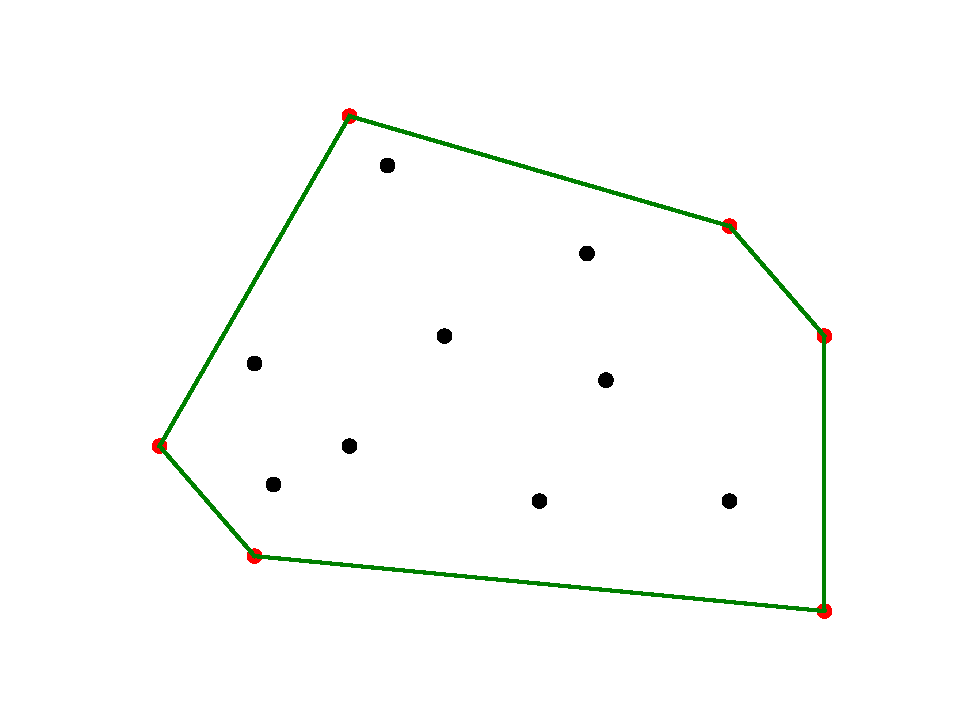
\includegraphics[width=0.8\textwidth]{convex_example.pdf}
    \caption{Conjunto convexo $X$. El anillo convexo de $X$ corresponen a los puntos rojos. Cada punto interior puede ser calculado como una combinación lineal de conv $X$ }
    \label{fig:convex_example}
\end{figure}

Sea $X \in \mathbb{R}^d$ un conjunto no vacio en un espacio de dimensión $d$. Asimismo $u : \bm{\mbox{conv}} X \rightarrow \mathbb{R}$ sea una función cuyos valores discretos son conocidos, y además sea solución al problema de Cauchy, se construye una aproximación $u^h$ de $u$ dada por la expresión, 
\begin{equation} \label{ec:1app} 
    u(\bm{x}) \approx u^h(\bm{x}) = \sum_i^n \alpha_i B_i (\bm{x}) = \bm{B}(\bm{x}) \bm{\alpha} 
\end{equation}
el vector $\bm{B}(\bm{x})$ denota la función de base (\textit{trial function}) y $\bm{\alpha}$ es el vector con los coeficientes de cada término de la función base, \textit{i.e.}, la función $u(x)$ se aproxima como una combinación lineal de una base vectorial $B_i : \bm{\mbox{conv}} X \rightarrow \mathbb{R}, \, i=1,\ldots,N$ con su factor $\alpha_i$ asociado. La idea consiste en escoger una función $\bm{B}(\bm{x}) \subseteq \mathbb{B}$ donde $\mathbb{B}(\bm{x})$ es el conjunto de funciones admisibles tal que $\bm{B}$ sean los coeficientes de conv $\hat{U}$ según la ecuación \ref{eq:convex_hull}. 
\begin{equation}
    \mathbb{B}(\hat{U}) = \left\{ B \in \mathbb{R}_+^N \; | \; \hat{\bm{U}} \bm{B} = u \; | \;  B_1 + \cdots + B_n = 1  \right\} 
\end{equation}
donde el conjunto $\hat{U}$ contiene los parámetros $\left\{ \hat{u}_1 \; \cdots \; u_n \right\}^T$ suponiendo además que $u \in \mbox{conv} \; \hat{U}$. Esto se abordará con más detalles en la Sección \ref{seccion:funciones_de_forma}


%%%%%%%%%%%%%%%%%%%%%%%%%%%%%%%%%%%%%%%%%%%%%%%%%%%%%

\subsection{Esquemas de formulación}
Los esquemas de formulación permiten plantear las ecuaciones gobernantes al interior del dominio y en sus contornos. Dentro de los cuales se encuentran la formulación débil y la formulación fuerte. Los principios utilizados en los métodos sin malla de formulación débil son similares a los abordado por el método de elementos finitos. En primer lugar la forma débil de la ecuación requiere de consistencias menos exigentes ya que se reduce en un grado la ecuación diferencial gobernante, además produce sistemas de ecuación más estables con resultados más precisos. 

%Existen variados maneras de generar ecuaciones con formulación débil, entre los más conocidos se encuetra el método de los residuos ponderados, el principio de Hamilton, principio de mínima energía potencial, el método de Galerkin (Galerkin Weak Form), entre otros, el lector podrá encontrar más detalles de cada uno de estos métodos en (PENDIENTE!). A continuación se describe el método residuos ponderados

%INVESTIGAR, QUE PASA CON PRINCIPIO DE HAMILTON, PRINCIPIO DE MÍNIMA ENERGÍA POTENCIAL, Y OTROS TIPOS DE APROXIMACIONES.
%
%Principio de Hamilton (Principio de mínima acción):
%-Principio variacional basado en el principio de energía
%-establece que: "of all possibles time histories of consistent displacement states wich satisfy:
%a. the compatibility conditions
%b. the essential (displacement or kinematical) boundary condition
%c. the condition at initial (t1) and final time (t2)
%the history corresponding to the actual solution makes the Lagrangian functional a minimal" :> admissible conditions
%Sea $L$ el funcional lagrangiano, el principio de Hamilton se expresa como
%\begin{equation}
%    \delta \int_{t_1}^{t_2} L dt = 0
%\end{equation}

%
%Una formulación fuerte de la ecuación que gobierna el fenómeno junto con sus condiciones de contorno establece que la solución debe satisfacer en cada uno de los puntos sobre el dominio. En cambio una formulación débil establece que la solución debe satisfacerse en sentido integral, en otras palabras, resuelve de manera \textit{promediada} la ecuación en un area acotada del subdominio local.
%
%Esto posee una implicancia en el grado de consistencia de de la función incognita $u(\bm{x})$, que permitan la diferenciación en el orden de la EDP. Por ejemplo, para una ecuación diferencial de $k^\circ$ orden, la formulación fuerte requiere que el campo nodal (o variable) posea continuidad de $k^\circ$ orden, mientras que un esquema de formulación débil necesita serlo de orden $(k-1)^\circ$. Esto se debe a que el operador integral reduce en un orden la derivada de la función incognita.


\subsubsection{Formulación débil}
La formulación variacional o débil consiste en la resolución de la forma integral de las ecuaciones gobernantes. Multiples alternativas permiten generar estas ecuaciones, (NOMBRAR OTRAS?). La forma de Galerkin se deriva del principio de Hamilton el cual establece que de todos los desplazamientos (infinitesimales) posibles que cumplan con las siguientes condiciones: a) Condiciones de compatibilidad (¿?), b) Condiciones de contorno, c) Condiciones temporales iniciales $t_1$ y finales $t_2$ (tambien conocidas como condiciones de admisibilidad), entonces aquel camino solución será aquel minimize el funcional Lagrangiano $L$, matematicamente establece que
\begin{equation} \label{eq:hamilton}
    \delta \int_{t_1}^{t_2} L \; dt = 0
\end{equation}
Por ejemplo en un sistema mecánico el funcional Lagrangiano corresponde a 
\begin{equation} \label{eq:energy_lagrangian}
    L = T - \Pi + W
\end{equation}
donde $T$ es la energía cinética, $\Pi$ es la energía de deformación y $W$ es el trabajo ejercido por una fuerza externa, estos términos se pueden expresar como
\begin{equation}
    T = \frac{1}{2} \int_{\Omega} \rho \dot{\bm{u}}^T \dot{\bm{u}} \; d\Omega
\end{equation}
\begin{equation}
    \Pi = \frac{1}{2} \int_{\Omega} \bm{\epsilon}^T \bm{\sigma} \; d\Omega
\end{equation}
\begin{equation}
    W = \int_{\Omega} \bm{u}^T\bm{b} \; d\Omega + \int_{\Gamma} \bm{u}^T \overline{\bm{t}} \; d\Gamma
\end{equation}
Reemplazando la ecuación \ref{eq:energy_lagrangian} en \ref{eq:hamilton} se obtiene
\begin{equation}
    \delta \int_{t_1}^{t_2} T - \Pi + W \; dt = 0
\end{equation}
es decir, un sistema mecánico sometido a fuerzas conservativas, el trabajo ejercido por un desplazamiento infinitesima debe ser nulo. Este principio se conoce como el principio de trabajo virtual o principio de mínima energía potencial. Notar que al aplicar esta formulación puede presentarse el caso que no se cumplan las condiciones de admisibilidad, particularmente en los puntos pertenecientes al contorno los cuales prescriban condiciones de dirichlet. Esta situación puede subsanarse modificando el funcional Lagrangiano agregando un termino adicional el cual permite imponer la condición en el contorno, utilizando para ello multiplicadores de Lagrange (citar) o el método de penalización. 

La formulación Galerkin es una de las más utilizadas en Elementos Finitos y en Métodos sin Malla. Para problemas de elasticidad lineal utilizando la relación de esfuerzo-deformación 
\begin{equation}
    \int_{\Omega} \delta (\bm{L}\bm{u})^T \bm{c} (\bm{L}\bm{u}) \; d\Omega - \int_{\Omega} \delta \bm{u}^T \bm{b} \; d\Omega - \int_{\Gamma} \delta\bm{u}^T \overline{\bm{t}} \; d\Gamma = 0
\end{equation}
Para solucionar los Más detalles acerca de las condiciones de admisibilidad van más allá del alcance de este trabajo. 

\subsubsection{Formulación fuerte}
Para generar una formulación fuerte del problema se recurre al Método de Residuos Ponderados (CITAR), el cual establece lo siguiente: Sea $\bm{u}=\bm{u}(\bm{x})$ función de $\bm{x} \in \Omega$, se considera la siguiente ecuación diferencial,
\begin{equation} \label{edp1} 
    \bm{F}(\bm{u}) - \bm{b} = 0 , \; \bm{x} \in \Omega 
 \end{equation}
\begin{equation} \label{edp2} 
\bm{G}(\bm{u}) - \bm{g} = 0 , \; \bm{x} \in \partial \Omega \end{equation}
donde $\bm{F}$ y $\bm{G}$ son operadores diferenciales que se aplican sobre $\bm{u}(\bm{x})$, las funciones $\bm{b}$ y $\bm{g}$ representan un campo diferencial sobre el dominio interior $\Omega$ y su contorno $\partial \Omega$, respectivamente.
\begin{equation} \label{2app} 
    \bm{u}^h(\bm{x}) = \sum_{i=1}^m \phi_i (x) \hat{u}_i = \bm{\phi}^T \hat{\bm{U}} 
\end{equation}
En general, reemplazando la aproximación \ref{2app} en \ref{edp1} y \ref{edp2} la igualdad no se cumple. Luego, se define la función de residuo (\textit{residual function}) como,
\begin{equation} 
\bm{R}_d = \bm{F}(\bm{u}^h) - \bm{b}  
\end{equation}
\begin{equation}
 \bm{R}_s = \bm{G}(\bm{u}^h) - \bm{g}  
\end{equation}
El método de residuos ponderados es una técnica que permite reducir el residuo. Se plantea la siguiente función.
\begin{equation} \label{eq:residuos_ponderados_1}
 \int_{\Omega} W_i \, \bm{R}_d \, d\Omega + \int_{\partial \Omega} V_i \, \bm{R}_s \, d\Gamma = 0 
 \end{equation}
\begin{equation} \label{eq:residuos_ponderados_2}
\int_{\Omega} W_i \, ( \bm{F}(\bm{u}^h) - \bm{b} ) \, d\Omega + \int_{\partial \Omega} V_i \, ( \bm{G}(\bm{u}^h) - \bm{g} ) \, d\Gamma = 0 
 \end{equation}
Donde $W_i$ y $V_i$ son funciones de ponderación o función de prueba (\textit{test function}) asociadas a $\bm{R}_d$ y $\bm{R}_s$ respectivamente. Este planteamiento permite reducir, en promedio, el error obtenido por la aproximación mediante el uso integral sobre el dominio y su contorno. La elección particular de $W_i$ y $V_i$ conduce a los distintos métodos de aproximación. Notar que cuando $W_i$ es igual a la función base $\bm{B}(\bm{x})$ de la ecuación (\ref{ec:1app}) se obtiene la formulación de Galerkin dada por (\ref{eq:Galerkin}) . Entre los más conocidos se encuentra el método de subdominios, el método de mínimos cuadrados, el método de momentos y el método de Galerkin. El método de Galerkin es ampliamente utilizado ya que desarrollo conlleva al mismo resultado obtenido principio de mínima energía, por lo que su implementación matemática además se condice con un fundamento físico, además de presentar un buen desempeño en la práctica. El principio de Galerkin establece lo siguiente:
El esquema de formulación propuesto es el colocación puntual (\textit{collocation point method}) \cite{liuintro} \cite{marchant} propone utilizar utilizar el delta de Krockener como:
\begin{equation} \label{deltaw} W_i = \delta(\bm{x}-\bm{x}_i) \end{equation}
\begin{equation} \label{deltav} V_i = \delta(\bm{x}-\bm{x}_i) \end{equation}
Reemplazando \ref{deltaw} y \ref{deltav} en \ref{residual}:
\begin{equation} 
\begin{split}
& \int_{\Omega} \delta(\bm{x}-\bm{x}_i) \, ( \bm{F}(\bm{u}^h) - \bm{b} ) \, d\Omega \\
& + \int_{\partial \Omega} \delta(\bm{x}-\bm{x}_i) \, ( \bm{G}(u^h) - \bm{g} ) \, d\Gamma = 0
\end{split} 
\end{equation}
Obteniendose el esquema de formulación fuerte,
\begin{equation}
 ( \bm{F}(\bm{u}^h) - \bm{b} ) + ( \bm{G}(\bm{u}^h) - \bm{g} ) = 0 
 \end{equation}
Notar que al utilizar el delta de Krockener la integral desaparece. Otros esquemas de formulación débil (donde no desaparece la integral) como el método del subdominio, de mínimos cuadradas, de momentos y de Garlekin \cite{liuintro}.

Cabe destacar que el método de colocación puntual cumple la propiedad de delta de Krockener, esto es,
\begin{equation}
\phi_i (\bm{x}=\bm{x}_j) = \left\{ 
\begin{matrix}
1 \, , \hspace{0,5cm} i=j\\
0 \, , \hspace{0,5cm} i \neq j
\end{matrix} \right.
\end{equation}
Como se explicó antes, el método de colocación puntual presenta inestabilidad, en especial en extremos con contorno tipo Neumann, para sobrellevar este problema existen métodos mixto que utilizando formulación fuerte en los nodos interiores y formulación débil en los extremos. Este tipo de esquema se llama formulación fuerte-débil.






























De manera general los métodos sin malla se puede clasificar según los criterios expuestos en la Tabla \ref{categoria}. \cite{liu-intro}

\begin{table}[H]
\centering
\begin{tabular}{p{3cm} p{8cm}}
\hline \hline
Clasificación & Categorias \\ \hline \hline
\multirow{4}{3cm}{Basado en procedimiento de formulación} & -Método basado en forma fuerte de la ecuación \\
 & -Método basado en forma debil de la ecuación \\
 & -Método basado en la combinación de forma fuerte-debil \\ \hline
\multirow{5}{3cm}{Basados en un método de interpolación/ aproximación} & -Método utilizando aproximación por mínimo cuadrados (MLS) \\
 & -Método utilizando representación integral \\
 & -Método utilizando interpolación puntual (PIM) \\
 & -Método utilizando utilizando otros métodos de interpolación \\ \hline
\multirow{3}{3cm}{Basado en representación del dominio} & -Métodos tipo dominio \\
 & -Métodos tipo contorno \\ & \\ \hline \hline
\end{tabular}
\caption{} \label{categoria}
\end{table}





%%%%%%%%%%%%%%%%%%%%%%%%%%%%%%%%%%%%%%%%%%%%%%%%%%%%%%%%

\section{Funciones de forma} \label{seccion:funciones_de_forma}

 se conoce como la función de forma asociada a un dominio acotado agrupados en el vector $\bm{\Phi}^T(\bm{x}) = \left\{ \phi_1(\bm{x}), \ldots , \phi_N(\bm{x}) \right\} $; y $ \bm{U_s}^T = \left\{ u_1, \ldots, u_N \right\} $ son los valores nodales de $u$ . 

Existen múltiples funciones que son solución de (\ref{uh_ecuacion_general}), al escoger una en particular se define un esquema de aproximación. La función de forma debe satisfacer la condición de consistencia de order cero (o partición de la unidad) y de primer orden, expresados respectivamente como:
\begin{equation} \label{0_orden_consistencia}
\sum_{i=1}^{N} \phi_i(\bm{x}) = 1 \hspace{0,5cm} \forall \bm{x} \in \bm{\mbox{conv}} X 
\end{equation}
\begin{equation} \label{1_orden_consistencia}
\sum_{i=1}^{N} \phi_{i}(\bm{x}) \bm{x}_i = \bm{x} \hspace{0,5cm} \forall \bm{x} \in \bm{\mbox{conv}} X 
\end{equation}
Estas condiciones garantizan que el esquema de aproximación reproduzca exactamente la función lineal. Si $N=d+1$ y el conjunto de puntos pertenecen a un espacio afín linealmente independiente, la condición de consistencia determina de manera única la función de forma sobre el correspondiente poliedro ($d$-simplex). En general $N > d+1$ por lo que adicionalmente se debe asegurar que la función de forma sea positiva,
\begin{equation}
\phi_i(\bm{x}) \geq 0 \hspace{0,5cm} \forall \bm{\mbox{conv}} X, \, i=1,\ldots,N
\end{equation} 
Por simple inspección se verifica que las propiedades exigidas a la función de forma $\bm{\phi}(\bm{x})$ son equivalente a las presentadas por la ecuación (\ref{eq:convex_hull}). Por lo tanto $\phi_i $ se puede interpretar como los coeficientes de una combinación convexa asociados a los $N$ valores nodales $u_i$.

\subsection{Mínimos cuadrados ponderados}

Una alternativa ampliamente utilizada para esquemas de colocación puntual es el método de mínimos cuadrados ponderados (\textit{Weighted Least Squares}), el cual plantea lo siguiente: Se desea aproximar la $u(\bm{x})$ mediante una base vectorial $\bm{p}$ tal que:
\begin{equation}
    u^h(\bm{x}) = \sum_{i=1}^m = p_i(\bm{x}) a_i(\bm{x}) = \bm{p}(\bm{x})^T \bm{a}(\bm{x})
\end{equation}
donde $p^T = \left\{ 1 \quad x \quad y \quad \cdots \quad p_m(\bm{x})\right\}$ y $\bm{a} = \left\{ a_1 \quad a_2 \quad \cdots \quad a_m\right\}$. La ecuación anterior es la expresión general del método de mínimos cuadrados moviles (\textit{Moving Least Squares} o MLS). Una alternativa consiste en considerar constante al parametro $\bm{a}$, este método se conoce como mínimos cuadrados fijos (\textit{Fixed Weighted Least Squares} o FWLS), es decir,
\begin{equation}
    u^h(\bm{x}) = \sum_{i=1}^m = p_i(\bm{x}) a_i = \bm{p}(\bm{x})^T \bm{a}
\end{equation}
donde $\bm{p}(\bm{x})$ es el vector base vectorial de grado $m$.
\begin{equation}
    \bm{p}(\bm{x}) = \begin{Bmatrix} 1 & x & x^2 \end{Bmatrix}
\end{equation}
\begin{equation}
    \bm{p}(\bm{x}) = \begin{Bmatrix} 1 & x & y & x^2 & xy & y^2\end{Bmatrix}
\end{equation}
\begin{equation}
    \bm{P}(\bm{x})  = \begin{bmatrix} \bm{p}(\bm{x}_1) \\ \bm{p}(\bm{x}_2) \\ \vdots \\ \bm{p}(\bm{x}_n) \end{bmatrix}
\end{equation}
\begin{equation}
    \bm{U}_s = \bm{P}(\bm{x}) \bm{a}
\end{equation}
\begin{equation}
    J = \sum_{i=1}^n W_i \left[ u^h(\bm{x}_i) - u(\bm{x}) \right]^2
\end{equation}
\begin{equation}
    \frac{\partial J}{\partial \bm{a}} = 0
\end{equation}
\begin{equation}
    \bm{P}^T \hat{\bm{W}} \bm{P} = \bm{P} \hat{\bm{W}} \bm{U}
\end{equation}
\begin{equation}
    \hat{\bm{W}} = \mbox{diag} \begin{bmatrix} w_1 & \cdots & w_n \end{bmatrix}_{n \times n}
\end{equation}
\begin{equation}
    \bm{A} = \bm{P}^T \hat{\bm{W}} \bm{P}
\end{equation}
\begin{equation}
    \bm{B} = \bm{P}^T \hat{\bm{W}}
\end{equation}
\begin{equation}
    \bm{a} = \left( \bm{P}^T \hat{\bm{W}} \bm{P} \right)^{-1} \left( \bm{P}^T \hat{\bm{W}} \right) U_s = A^{-1} B U_s
\end{equation}
\begin{equation}
    u^h(\bm{x}) = \bm{p}^T \bm{a} = \bm{p}^T \bm{A}^{-1} \bm{B} \bm{U}_s = \bm{\Phi}^T  \bm{U}_s
\end{equation}
\begin{equation}
    \bm{\Phi}^T = \bm{p}^T \bm{A}^{-1} \bm{B} = \begin{Bmatrix} \phi_1 & \cdots & \phi_n \end{Bmatrix}
\end{equation}




%%%%%%%%%%%%%%%%%%%%%%%%%%%%%%%%%%%%%%%%%%%%%%%%%%%%%%%%

\section{Diferencias entre FEM y MESHFREE}

El Método de Elementos Finitos (\textit{Finite Elements Method, FEM}), es un método robusto ampliamente estudiado. Es versatil ya que es flexible frente a problemas lineales y no lineales y puede ocuparse en geometrías complejas. Generalmente \textit{FEM} se utiliza para problemas de sólidos y estructuras.

Sin embargo, el método presenta ciertas desventajas, todas ellas debido a la necesidad de disponer de un malla \textit{a priori}:
\begin{enumerate}
\item Alto costo en la generación de la malla. La resolución de problemas implica la creación de la malla (discretización del dominio) y la resolución de las ecuaciones resultantes. Usualmente se emplea más recursos computacionales en la generación de esta malla. Esto trae consigo otro inconveniente:
\item Dificultad en el análisis adaptativo. Para asegurar la exactitud del método se requiere que el análisis empleando FEM \textit{reconstruya} la malla, de tal manera de asegurar una conectividad apropiada entre los elementos.
\item Otros problemas donde se presentan dificultades:
\begin{itemize}
\item Problemas que presentan grandes deformaciones tienen una considerable pérdida de exactitud
\item Es dificil simular el fenómeno de propagación de grietas en recorridos que con coinciden con la interface de los elementos discretos
\item FEM está basado en la teoría de mecánica de medios continuos, por lo que es dificil simular la fractura de material con un gran número de fragmentos (el elementos debe mantenerse, o bien, desaparecer por completo)
\end{itemize}
\end{enumerate}

Por otro lado, los métodos sin malla discretizan el dominio utilizando nodos (o partículas) que interactuan unas con otras mediante una función de forma. Al prescindir de una malla el método se vuelve flexible, aplicable a problemas de fluidos y de sólidos sometidos a grandes deformaciones.

Las ventajas más importantes de los métodos Meshfree son su alto grado de continuidad de su función de forma; Mayor suavidad (\textit{smoothness}) de la modelación; Presenta ventaja al momento de modelar problemas de fractura, entre otros.

Las desventajas más importantes que presentan estos métodos son, en general, su mayor costo computacional y la inestabilidad que posee algunas de estos formulaciones.

A pesar de presentar importantes aplicaciones actualmente están en una etapa de desarrollo. Existe una línea de investigación orientada a resolver problemas técnicos de estos métodos para volverlo una herramienta robusta.

%%%%%%%%%%%%%%%%%%%%%%%%%%%%%%%%%%%%%%%%%%%%%%%%%%%%%%%%%%%%

\section{Métodos numéricos} \label{cap2}

%FEM
El Método de Elementos Finitos (\textit{Finite Elements Method, FEM}), es un método robusto ampliamente estudiado. El método consiste en dividir un contínuo en varios elementos finitos (discretización) conectados de una manera predefinida (malla). Es versatil ya que es flexible frente a problemas lineales y no lineales y puede ocuparse en geometrías complejas. Generalmente \textit{FEM} se utiliza para problemas de sólidos y estructuras. Además de existir paquetes de software ampliamente utilizados y desarrollados.

%Meshfree
Los métodos sin malla se definen como \textit{un método utilizado para establecer un sistema algebraico de ecuaciones para un dominio de un sistema sin utilizar una malla predefinida en de la discretización del dominio}. Esta metodología utiliza un conjunto de nodos dispersos tanto dentro del dominio del problema como en su contorno. Como estos puntos no forman parte de una malla no requieren información \textit{a priori} entre los nodos de interpolación. Las ventajas más importantes de los métodos Meshfree son su alto grado de continuidad de su función de forma, poseer mayor suavidad (\textit{smoothness}) de la modelación.

Una de las principales motivaciones para trabajar con métodos sin malla derivan de ciertas desventajas que se presentan al momento de disponer de una malla \textit{a priori}, algunas de estas limitaciones son \cite{liuintro}: Alto costo en la generación de la malla. La resolución de problemas implica la creación de la malla (discretización del dominio) y la resolución de las ecuaciones resultantes: La generación de la malla contempla cerca del $20\%$ del tiempo total del análisis y la posterior adaptabilidad de la misma (osea, creación de una geometría adecuada para el análisis) requiere cerca del $60\%$ del tiempo, y solo el $20\%$ del tiempo total de cómputo empleado va destinado a análisis \textit{per se}\cite{IGA_LIBRO}. Esto trae consigo otro inconveniente: Dificultad en el análisis adaptativo. Para asegurar la exactitud del método se requiere que el análisis empleando FEM \textit{reconstruya} la malla, de tal manera de asegurar una conectividad apropiada entre los elementos.

Otros problemas donde se presentan dificultades:
\begin{itemize}
\item Problemas que presentan grandes deformaciones tienen una considerable pérdida de exactitud
\item Es dificil simular el fenómeno de propagación de grietas en recorridos que con coinciden con la interface de los elementos discretos
\item FEM está basado en la teoría de mecánica de medios continuos, por lo que es dificil simular la fractura de material con un gran número de fragmentos (el elementos debe mantenerse, o bien, desaparecer por completo)
\end{itemize}

%PROBLEMAS CON MESHFREE
Luego, los métodos meshfree suponen una ventaja comparativa con respecto metodos con malla, como FEM. Sin embargo, algunas de las desventajas más importantes que presentan estos métodos son, en general, su mayor costo computacional y la inestabilidad que posee algunas de estos formulaciones.

%%%%%%%%%%%%%%%%%%%%%%%%%%%%%%%%%%%%%%%%%%%%%%%
%%%%%%%%%%%%%%%%%%%%%%%%%%%%%%%%%%%%%%%%%%%%%%%
%ESTADO DEL ARTE
%%%%%%%%%%%%%%%%%%%%%%%%%%%%%%%%%%%%%%%%%%%%%%%
%%%%%%%%%%%%%%%%%%%%%%%%%%%%%%%%%%%%%%%%%%%%%%%

%ALGUNOS PAPERS DE MF

Respecto a métodos de colocación puntual o formulación fuerte cabe nombrar algunos estudios. Se utiliza un método de colocación puntual utilizando polinomios de Chebyshev (método pseudoespectral) para resolver numericamente problemas de solidificación direccional \cite{solidification}. Este tipo de planteamientos contemplan superficies fluidas o interfaces sólido-líquido, y su aplicación tecnológica está orientada a procesos que involucran crecimiento de cristales, congelamiento y derretimiento y propagación de llamas.

Se han utilizado además en la resolución de la ecuación de Navier-Stokes (stream-vorticity formulation) en dos dimensiones utilizando el método \textit{Fast Moving Least Squared Approximation} (FMLS) \cite{2D_NS_MF} obteniendo resultados favorables ya que los métodos de colocación cumplen con la propiedad de delta de Krockener, pudiendo imponer condiciones esenciales en los contornos. Cabe destacar algunas aplicaciones de métodos sin malla en el área de la neurociencia: En \cite{eeg} utiliza un método de colocación puntual (finite point method) con función de forma basada en mínimos cuadrados, prefiriendose este método debido a la alta demanda de cómputo que exige FEM y BEM\footnote{BEM: Boundary element method}

%%%%%%%%%%%%%%%%%%%%%%%%%%%%%%%%%%%%%%%%%%%%%%%
%MAXENT
%%%%%%%%%%%%%%%%%%%%%%%%%%%%%%%%%%%%%%%%%%%%%%%

\subsubsection{Máxima entropía en métodos sin malla}

Se establece una relación entre la mecánica estadística y la teoría de la información \cite{jaynes}. Esta última provee criterios para construir distribuciones de probabilidades en base de la información parcial conocida, lo que lleva a un tipo de inferencia estadística llamada estimador de maxima entropía \cite{shannon}. Jaynes en su estudio considera a la mecánica estadística como una forma de inferencia estadística. (mecánica estadística 'subjetiva' cuyas consideraciones no contemplan argumentos físicos, siendo aún así la mejor estimación con los datos disponibles).

la máxima entropía se pueden entender como una técnica para estimar la probabilidad de un evento en forma generalizada. Como resultado de este principio se obtiene una distribución de probabilidad del evento a estudiar, considerando las restricciones probabilisticas del problema.  La solución obtenida de esta manera tiene como característica principal poseer \textit{la menor incertidumbre posible para la información disponible}.

En respuesta de los anterior se ha propuesto en los décadas la implementación de este principio en diversos problemas, entre ellos, para idear un esquema de aproximación para métodos sin malla. Se tiene que esta formulación maxent arroja valores estrictamente positivos, esta es una característica buscada al momento de escoger funciones de forma ya que le da el sustento matematico a que el método realmente aproxima la función en un dominio covexo. En \cite{arroyo} se expone un esquema de aproximación local utilizando el principio maxent considerando la triangulación Delanauy en la utilización de métodos sin malla de formulación débil. Se utiliza el funcional de máxima entropía para solucionar problemas derivados de la degeneración en la triangulación utilizando (esto sucede cuando la triangulación no es única, luego se busca una solución optima mediante la resolución del problema dual de optimización). Recientes investigaciones han propuestos esquemas similares al anterior, pero utilizando el ánalisis isogeométrico utilizando aproximantes utilizando maxent local \cite{IGA_LME}. El análisis isogeométrico corresponde a un método que \textit{fusiona} el estudio geométrico y analitico de un problema, es decir, permite integrar las funciones de forma (que gobiernan el problema) con el modelamiento CAD mediante la utilización de NURBS\footnote{NURBS: non-uniform rational B-spline} (ver Figura \ref{3})   %(HUGHES) primera publicación del IGA

Tambien se ha utilizado en métodos meshfree basado en maxent en problemas de sólidos incompresibles y cuasi-incompresibles\cite{maxent_en_elasticidad}. En dicho trabajo se presentan dos situaciones: Errores numericos inducidos por la integración y el fenomeno de 'volumetric locking'. El primero de estos casos proviene del hecho que los métodos de formulación débil requieren de una malla de integración (background cell for integration) por lo que se plantean métodos modificados de integración (\textit{modified Gaus integration}). En \cite{marchant} se realiza una comparación el comportamiento entre la función de forma de máxima entropía y minimo cuadrado ponderado fijo (FWLS) en la resolución de ecuaciones elípticas  de segundo orden (Test de Rachford-Wheeler). Ahí se plantea el problema de optimización convexa aplicado a metodos de formulación fuerte. Se observa que maxent converge con mayor rápidez que FWLS, además se observa que los resultados presentan una mejora en la exactitud al momento de resolver el test sometido a condiciones de contorno tipo Neumann. Esto da indicios que maxent puede representar una solución a la inestabilidad que presentan los métodos de colocación puntual frente a estas condiciones. Una de las razones de este desempeño se debe a que maxent es una función positiva (ver Figura \ref{1})

